\documentclass{standalone}

\begin{document}

\chapter*{Appendix C - BlendNet}\addcontentsline{toc}{chapter}{Appendix C - BlendNet}
\markboth{Appendix C}{BlendNet}

\begin{figure}[htbp]
\centering
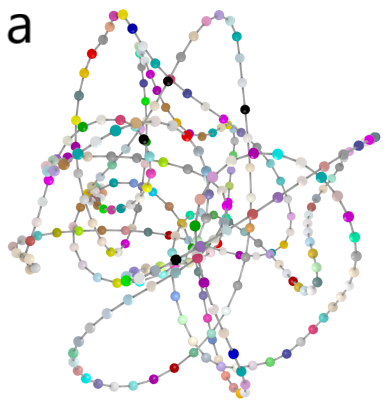
\includegraphics[width=0.4\textwidth]{cycle_graph.png}
\qquad\qquad
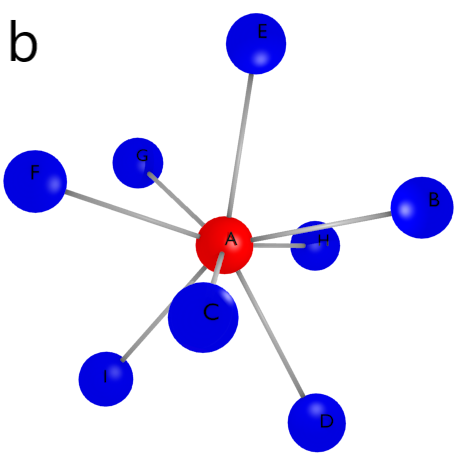
\includegraphics[width=0.4\textwidth]{star_graph_node.png}
\caption{(\textbf{a}) Chain graph rendered by \textsf{BlendNet} software.
Node colors are randomly generated by the tool.
(\textbf{b}) Star graph rendered by \textsf{BlendNet} software.
Node colors and labels are given as extra columns in node-list file.
}
\label{fig:blendnet}
\end{figure}

Graph visualization is still an open problem in many applications.
The problem is commonly related to large graph visualization in which problems arise from the rendering of a large number of nodes and a greater number of links between them (a graph with $N$ nodes could have $(N \times N)$ possible links).
An other open problem concern the multi-dimensional visualization of the graphs.
Despite common graph tools compute the node coordinates in any space dimensions (and clearly the maximum number of possible dimensions for a visualization is only 3) the real visualization is often allowed only in 2D spaces.
The counterpart of these problems concern a pretty visualization of the graphs, that it is often ignored by many tools which prefer focusing on simple renderings.

In this section we introduce a new custom graph viewer developed for pretty small-networks visualization in 2D and 3D, called \href{https://github.com/Nico-Curti/BlendNet}{\textsf{BlendNet}}~\cite{BlendNet} (\emph{Blender Network viewer}).
\textsf{BlendNet} is an open-source project and it is released on Github under GPL license.
All the small-graphs showed in this work are made using this tool and in particular the feature-signatures generated by the \textsf{DNetPRO} algorithm.

\textsf{BlendNet} is written in \textsf{Python} with the help of \textsf{Blender} APIs.
\textsf{Blender} is now a standard for 3D rendering and it is commonly used in a wide range of graphical applications, starting from the simpler 3D dynamics to video-game applications.
\textsf{Blender} is certainly more than a simple graphical viewer, but it provides an easy \textsf{Python} interface and a wide on-line documentation which make it a useful tool for graphical representation of 3D structures.

We are forced to use the \textsf{Python} version provided by \textsf{Blender} to use its APIs and any extra-package required by our application has to be installed with the appropriated \textsf{pip}.
We use the \textsf{networkx} \textsf{Python} library for node coordinates computation and thus we have to update our \textsf{Python}-\textsf{Blender} with the appropriated packages.
Moreover, since the code can be difficult to manage for non-expert users, we have written an easy command-line interface to set the whole set of parameters required by the graph viewer that can be piloted via \href{https://github.com/Nico-Curti/BlendNet/blob/master/Makefile}{\textsf{Makefile}} rules.
The list of nodes and edges can be passed via command-line with the relative filenames, in the same format of the concurrent graph viewers (e.g \emph{Gephi} software, the other graph viewer used in this work to generate the larger network structures of the \textsf{CHIMeRA} project).

The software project is a single script file and it includes a full list of possible \href{https://github.com/Nico-Curti/BlendNet/blob/master/example}{examples} and usages.
Some of this examples are shown in Fig.~\ref{fig:blendnet}.
A full list of installation instructions is also provided for any operative system (\href{https://github.com/Nico-Curti/BlendNet/blob/master/install.sh}{Unix, MacOS} and \href{https://github.com/Nico-Curti/BlendNet/blob/master/install.ps1}{Windows}).
These instructions cover a full installation of \textsf{Blender}, \textsf{Python} and \textsf{BlendNet} package for administrator and no-root users (ref. \textsf{Shut} project \cite{Shut}).
With slight code editing we can obtain different node coordinates and shapes.
Node colors, sizes and positions can also be given using the node-list file as independent columns.

\end{document}
